\chapter{Results and Analysis WHAT}
\label{chp:results}
\section{On the content}
\section{Survey results}
\label{chp:surveyResults}
Looking at the survey results, we can see that our algorithm won $\frac{2}{3}$ of the times, as can be seen in figure \ref{fig:surveyOverall}. This indicates that our algorithm is more suitable for finding highlights for certain types of players. Most of the respondents were very familiar with the game, showing that experienced players seemed to like our implementation.
\begin{figure}
\centering
\begin{tikzpicture}[object/.style={thin,double,<->}]
 \pie{66.6/Our algorithm,33.3/Allstar} 
\end{tikzpicture}
\caption{Pie chart showing what algorithm won in the survey}
\label{fig:surveyOverall}
\end{figure}
\subsection{Match 1}
\textbf{old text}
In the first match, our algorithm just took the win. It is not a large win by any stretch of the imagination, but based on the comments added by the respondent, both highlights are very close. However, a respondent said that Video A was more tactical, but that both clips were clean. Another user, who preferred Video B, said that that play was more fearless. The people that choose B seemed to think video B has more action and better decision making. The people who chose A commented on how \gls{clean} it was

For this set of highlights, video A won by a slim margin. The people that taught video a was the better one commented on that it was more tactical and \gls{clean}. That the AK47 was used instead of the glock also attracted some viewers. One respondent said that; "It was a good clutch". The respondents that liked video B had the opinion that that highlight had more action. The people who responded indifferently mentioned that both clips were the same in terms of level of game play.

\textbf{URLS HERE}
\begin{figure}
\centering
\begin{tikzpicture}[object/.style={thin,double,<->}]
 \pie{40/ Video A (Our algorithm),36/Video B (AllStar), 24/Indifferent} 
\end{tikzpicture}
\caption{Result from Match 1}
\label{fig:match1}
\end{figure}


\subsection{Match 2}
For this set of highlights, video B took the win, with a little more than half of the respondents liking this highlight more. Respondents mentioned that the knife kill during video B was a large factor, and that the kills were all solo plays, with no help from teammates. They also mentioned that video A was more messy and video B was more clean.


\textbf{URLS HERE}
\begin{figure}
\centering
\begin{tikzpicture}[object/.style={thin,double,<->}]
 \pie{34.6/ Video A (Our algorithm),57.7/Video B (AllStar), 7.7/Indifferent} 
\end{tikzpicture}
\caption{Result from Match 2}
\label{fig:match2}
\end{figure}
\subsection{Match 3}
For this set of highlights Video B was the winning highlight. While several viewers liked the impressive 4K spraydown and first kills in Video A, the majority found the gameplay in Video B to be better.

Some comments highlighted specific reasons why Video B was more appealing.

\begin{itemize}
\item \textbf{Better decision-making:} One respondent said that "The Read on The Game is on the 2nd Video way more accurate."
\item \textbf{Map awareness:} Another respondent said "Better checks on corners."
\item \textbf{Overall gameplay:} Several viewers simply stated their preference for Video B, indicating a more enjoyable viewing experience.
\end{itemize}

\textbf{URLS HERE}
\begin{figure}
\centering
\begin{tikzpicture}[object/.style={thin,double,<->}]
 \pie{65.4/ Video B (Our algorithm),19.2/Video A (AllStar), 15.4/Indifferent} 
\end{tikzpicture}
\caption{Result from Match 3}
\label{fig:match3}
\end{figure}
\subsection{Match 4}


For this set of highlights Video B was the winning highlight for a few reasons.

\begin{itemize}
\item \textbf{Fast-paced action:} One respondent stated, "Video B was way fast paced, which I like more."
\item \textbf{Strategic gameplay:} One respondent commented: "Just a better round, he knows what he is doing and plays around the enemies making mistakes" which shows a more calculated approach to the game.
\item \textbf{Map control:} Another viewer noted that "Video B felt like it opened up an A push pretty cleanly," showing that taking initiative, and opening up a site makes a good highlight.
\end{itemize}

Overall, viewers found Video B to be a better highlight, due to its faster and more strategic gameplay. The criticism of Video A mentioned a hesitation to push forward, and some bad mechanics regarding jump spotting.
\textbf{URLS HERE}
\begin{figure}
\centering
\begin{tikzpicture}[object/.style={thin,double,<->}]
 \pie{50/ Video B (Our algorithm),42.3/Video A (AllStar), 7.7/Indifferent} 
\end{tikzpicture}
\caption{Result from Match 4}
\label{fig:match4}
\end{figure}
\subsection{Match 5}


People liked Video B more in this set of highlights.
The reasons that the respondents liked video B more:

\begin{itemize}
\item \textbf{Used smoke well:} "Played the smoke (very nice!) on video B"
\item \textbf{Got more kills:} "In video B he does not die, and gets most of the kills"
\item \textbf{Won the round:} "He didnt die, and won round"
\end{itemize}

While some people liked the skills shown in Video A, most preferred Video B because the player made good choices and won their team the round, as well as he did not die.
\textbf{URLS HERE}
\begin{figure}
\centering
\begin{tikzpicture}[object/.style={thin,double,<->}]
 \pie{57.7/ Video B (Our algorithm),34.6/Video A (AllStar), 7.7/Indifferent} 
\end{tikzpicture}
\caption{Result from Match 5}
\label{fig:match5}
\end{figure}
\subsection{Match 6}

Most people liked Video B more, saying it had cleaner kills. Some people liked Video A because it was fast-paced and showed teamwork.

The difference between the highlights were:
\begin{itemize}
\item \textbf{Video A - Fast and teamwork:} Some respondents liked how Video A was quicker and showed the whole team working together.
\item \textbf{Video B - Cleaner kills:} Others thought the kills in Video B looked nicer and smoother.
\end{itemize}

A few respondents said both videos were good and bad in different ways. Some also mentioned the teamkills during that round.

\textbf{URLS HERE}
\begin{figure}
\centering
\begin{tikzpicture}[object/.style={thin,double,<->}]
 \pie{38.5/ Video A (Our algorithm),46.2/Video B (AllStar), 15.4/Indifferent} 
\end{tikzpicture}
\caption{Result from Match 6}
\label{fig:match6}
\end{figure}
\subsection{Match 7}
The survey results shows that people liked Video A more. Video A had more kills, including a cool 2-kill spraydown, and the player got the last kill. Some people also liked that it was faster-paced.

\begin{itemize}
\item \textbf{More kills and a cool spray:} "More kills, aswell as a nice 2K spraydown."
\item \textbf{Got the last kill:} "He made the last kill himself in Video A liked that better."
\item \textbf{Faster pace:} "it was also way more fast paced."
\end{itemize}

Some people liked Video B and thought the player made smarter choices, but overall, Video A was more popular.
\textbf{URLS HERE}
\begin{figure}
\centering
\begin{tikzpicture}[object/.style={thin,double,<->}]
 \pie{46.2/ Video B (Our algorithm),38.5/Video A (AllStar), 15.4/Indifferent} 
\end{tikzpicture}
\caption{Result from Match 7}
\label{fig:match7}
\end{figure}
\subsection{Match 8}
The survey shows that video A was the preferred highlight, particularly for the clutch situation, cleaner kills, and higher kill count. While Video B was liked for its efficient 3K, some respondents noted the opponent's missed AWP shots as a huge reason that the highlight even was possible.

\begin{itemize}
\item \textbf{Video A's clutch and kills:} Several viewers favored Video A for the player's ability to secure kills in a clutch situation and the overall higher kill count.
\item \textbf{Video A's cleaner kills:} Some viewers specifically mentioned that the kills in Video A were cleaner and more impressive.
\item \textbf{Video B's methodical 3K:} While acknowledging the skill involved in the 3K in Video B, viewers also pointed out the opponent's missed AWP shots was the only reason this highlight was possible.
\end{itemize}

Overall, the respondents liked Video A for its clutch, and higher kill count and overall was cleaner and Video B was liked for its systematic approach even tho some luck was involved.
\textbf{URLS HERE}
\begin{figure}
\centering
\begin{tikzpicture}[object/.style={thin,double,<->}]
 \pie{65.4/ Video A (Our algorithm),26.9/Video B (AllStar), 7.7/Indifferent} 
\end{tikzpicture}
\caption{Result from Match 8}
\label{fig:match8}
\end{figure}
\subsection{Match 9}

Video B won here due to its better game sense, and that it was fast-paced. The highlight was long and showed that it took a long time for the player to win the round.
The reasoning given from the respondents were:

\begin{itemize}
\item \textbf{Video B's better kills:} Multiple viewers highlighted Video B's better kills, with one specifically mentioning the "clean glock 2K."
\item \textbf{Fast-paced action:} Viewers enjoyed the fast pace of Video B, particularly the initial kills.
\end{itemize}
\textbf{URLS HERE}
\begin{figure}
\centering
\begin{tikzpicture}[object/.style={thin,double,<->}]
 \pie{26.9/ Video A (Our algorithm),61.5/Video B (AllStar), 11.5/Indifferent} 
\end{tikzpicture}
\caption{Result from Match 9}
\label{fig:match9}
\end{figure}

\section{How can one create an algorithm to find better highlights in Counter Strike 2}
The first thing one needs to do is to figure out what metrics should be included in the algorithm. Here, you could interview people in the scene with experience, like casters, analysts, and players of the game. You can also study popular highlights from the community, and see what metrics are the highest in the highlights you watched, and use that as a baseline for what metrics are important to include in highlights. 

Next step in the process to create an algorithm for highlights is to extract the data. Here there is a few approaches that you can take. There is the approach that we took, which is implementing a parser step, to extract all relevant data from the demo file, and gives it into an workable format for the algorithm. Another way to do this is to analyze the video feed from either a screen capture or from a video file. This would require looking at properties of the video / stream, for example watching the kill feed or chat with OCR, and extract data from that, as well as other game information from the UI. Another approach is to use Counter Strike game state integration to get the data in real time from the game itself during the match. This would allow taking a clip of the user screen instead of having to render the clip on a separate server. The game state integration provides much the same data as a demo file would, but in real time.

Once the data has been collected, you would need to analyze that somehow. This is the most "free" part. Depending on what you want to include in the highlights, this will differ a lot. In our case, we focused on mechanical plays, like kills and the skill of the player, but another way would be to focus on funny plays.

Once this is done, the last part is to output the round number of the highlight, and what player did the highlight. Processing this and rendering the highlight is outside the scope of this algorithm.
\section{What metrics are most important when developing an algorithm to find highlights in Counter Strike 2}
To find what metrics, that are important for Counter Strike 2 highlights, we conducted interviews. In these interviews, we got different results:
\paragraph{What is your experience with Counter-Strike or other FPS games?}
2 out of the 7 had little to no experience with the game Counter Strike, but 6 out of 7 had played similar games.
\paragraph{What is your experience with highlights in FPS games?}
2 out of the 7 interviewees had no experience with highlights from FPS games.\\\\
\paragraph{What do you think is the most memorable highlight in Counter Strike history?}
6 out the 7 interviewees answered this question:
\begin{itemize}
    \item "I think the happy 1Deag ace on Banana" (Participant B1, personal communication, April 21, 2024)
    \item "Yes absolutely. After all, I have both famous ones from big tournaments or matches like Coldzera when he jumps and shoots on Mirage."(Participant L1, personal communication, April 10, 2024)
    \item "When you get a four K. It's cool stuff like that." (Participant O1, personal communication, April 30, 2024)
    \item "I think that when you kill a whole team, that's like you just rampage." (Participant O2, personal communication, April 16, 2024)
    \item "But if I'm off the cuff, what pops into my head is Hiko. When he was clutching Dust 2 or something like that."(Participant A1, personal communication, April 09, 2024)
    \item "It's probably OlofPass actually. Because then I was there when he made that boost."(Participant J1, personal communication, April 26, 2024)
\end{itemize}
\paragraph{What makes it memorable?}
Those who mentioned a specific clip said:
\begin{itemize}
    \item "The casters. Caster. Yeah. I suppose also the importance of the round." (Participant B1, personal communication, April 21, 2024)
    \item "The important thing is either that it is some kind of personal reference. That it's someone you know that you play with or that you watch that you know or something. Or that there is something big at stake, like a big tournament, big match or professional team. Then it will be memorable right away." (Participant L1, personal communication, April 10, 2024)
    \item "For me, that's what makes a good highlight. Precisely the part that lifts it is the skill demonstration. But also when the commentator is so damn hyped. That combination to me is absolutely fantastic. You get a lot of everything. If it's not from the clip, it's from the commentator. This for me means a lot. Unless there is no caster. Which it is not when you play yourself. Then music can be the supporting part. That you have music that is timed with the shot or similar." (Participant A1, personal communication, April 09, 2024)
    \item "It was that one that caused so much speculation and everything afterwards. The players had no idea it was super controversial and all. There is also a P3 documentary about this. Just that specific event. And then that it was also ten years ago and that it is still very, very memorable. And then that he is Swedish too." (Participant J1, personal communication, April 26, 2024)
\end{itemize}
\paragraph{What makes a good highlight?}

\begin{itemize}
    \item "Quick succession. Quick responses. Like going from one to the other in rapid succession. And quantity of kills usually." (Participant B1, personal communication, April 21, 2024)
    \item "Yes, but it is something that is either completely improbable, insanely difficult to succeed with" (Participant L1, personal communication, April 10, 2024)
    \item "But it's clips like this where you beat all the odds and manage to clutch a round. Or then something funny happens that causes you to drop from heaven on nuke and then you die. And then the others win." (Participant L1, personal communication, April 10, 2024)
    \item "A good highlight is made when there are a lot of people watching at the same time when a good commentator at a professional match does a lot. And the circumstances, such as the thing that he is in Sweden and does such a thing against a non-Swedish team, means that everyone gets extra hyped." (Participant J1, personal communication, April 26, 2024)
    \item "And the best is probably if it's one against five or similar so that everyone can see you when you play." (Participant J1, personal communication, April 26, 2024)
    \item "It could be a skill demonstration of how to aim your crosshair. It can be your movement in the game. It doesn't have to be that you bunny hop on mirage to short. It could just be that you're timing nicely. That you read the opponents. That you let people pass. There is so much that can make a good highlight. I have a hard time pointing to a thing. But if I have to point to one thing, it's one taps. I think that is absolutely fantastic. I think that is always worth including in a highlight. Deagle OneTaps. It could be AKs. If you do it several times in the same round or you have 5 kills via OneTaps." (Participant A1, personal communication, April 09, 2024)
    \item "But I think the technical stuff." (Participant E1, personal communication, April 14, 2024)
    \item "It must be something cool that happened. The more kills the better. The faster the guys, the closer the guys are to each other, the better. The more shady the weapon if you do something cool with it the better." (Participant O1, personal communication, April 30, 2024)
    \item "So if you dodge around a corner or something or have to do a lot of shit to get to the kill itself, that's more impressive." (Participant O2, personal communication, April 16, 2024)
\end{itemize}

\paragraph{Rate these metrics from 1-10:}\todo{move over pictu}

    \begin{figure}[H]
        \centering
        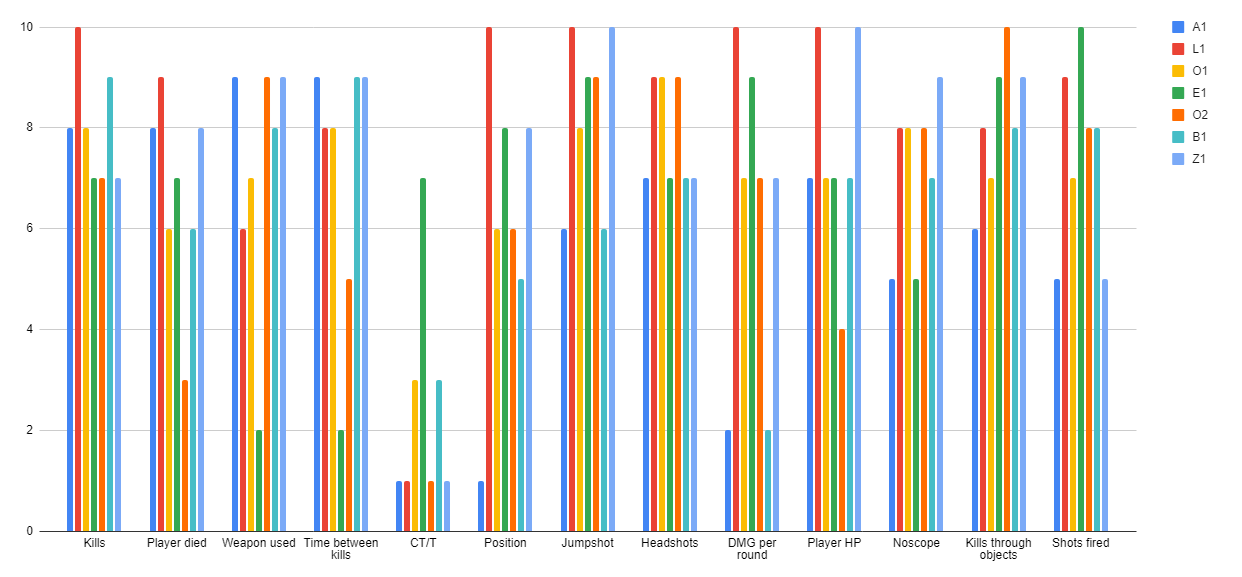
\includegraphics[width=17cm]{Images/All_results.png}
        \caption{Results from metrics rating}
        \label{fig:Barchart}
    \end{figure}
    \begin{figure}[H]
        \centering
        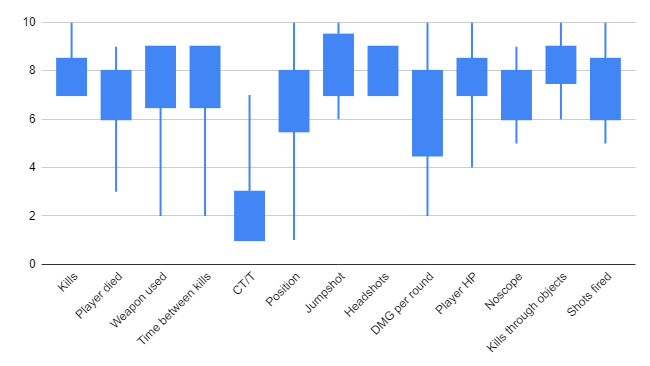
\includegraphics[width=17cm]{Images/boxplot.png}
        \caption{Box plot metrics}
        \label{fig:BoxplotMetrics}
    \end{figure}
    \begin{figure}[H]
        \centering
        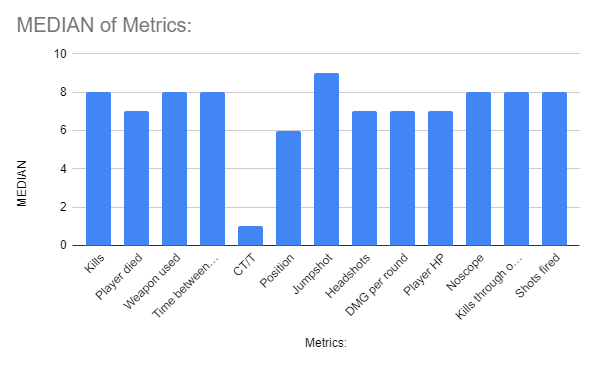
\includegraphics[width=17cm]{Images/medianMetrics.png}
        \caption{Median of metrics}
        \label{fig:medianMetrics}
    \end{figure}
    \textbf{Are there any metrics we forgot?}
    \begin{itemize}
        \item "After all, it is to create a metric to start running highlights when enemies are close to each other. Like in smokes or distance wise. Because if you are very close to each other on a site or something, highlights are rarely created there." (Participant L1, personal communication, April 10, 2024)
        \item "Well, hit percentage of the amount of bullets fired, right? I'm thinking, well, more or less. Oh, one second. Yeah, no, that's about it. The hit ratios are important to me. And maybe crosshair placement." (Participant B1, personal communication, April 21, 2024)
        \item "Kind of like Olofboost there." (Participant J1, personal communication, April 26, 2024)
        \item "Something you didn't mention was this movement thing." (Participant A1, personal communication, April 09, 2024)
        \item "Real movement players." (Participant O1, personal communication, April 30, 2024)
    \end{itemize}
\paragraph{Do you use any tool to create highlights?}
\begin{itemize}
    \item "I don't use anything. If I were to do it, I would use something that was simple and fast. Which fixed nice highlights. Which I could save and display. So, share those that might be able to be sent on discord directly. Or similar. Like GIFS." (Participant L1, personal communication, April 10, 2024)
    \item  "Yeah, FaceIt, like the FaceIt one." (Participant B1, personal communication, April 21, 2024)
    \item "And I use medal just to do it manually."(Participant B1, personal communication, April 21, 2024)
    \item "No, no more than the automatic that comes, for example, on e-sportal or results or something like that." (Participant J1, personal communication, April 26, 2024)
    \item "And then there's also GeForce Experience as well." (Participant J1, personal communication, April 26, 2024)
    \item "I used Medal around a year and a half ago. Then there was a lot of recording" {aiimar}
    \item "Leetify" (Participant O1, personal communication, April 30, 2024)
    \item "Yeah, Gif your game. Gif your game, but that's all." (Participant O2, personal communication, April 16, 2024)
    
\end{itemize}

\section{How do the perception of what makes a good highlight differ between novice and experienced players}
In the interviews, the biggest difference between novice and experienced players was in the specificity of the answers, those with less experience had a harder time explaining what they liked in a highlight. There was also less real life examples of highlights from those who had less experience.

